\documentclass[a4paper,french,12pt, titlepage]{article}

%%%% paquetages %%%%
\usepackage[french,english]{babel}  %définition de la langue
\usepackage[T1]{fontenc}
\usepackage[utf8]{inputenc} %définition de l'encodage
\usepackage{fullpage} %pour réduire les marges
\usepackage{graphicx} %pour figures
\usepackage{comment}
\usepackage{xcolor}
\usepackage{listings}
\usepackage{amsmath}
\usepackage{tikz}
\usepackage{hyperref}
\usepackage{wrapfig}
\usepackage{fancyhdr} %headers
\usepackage{glossaries}
\usepackage{todonotes}
\usepackage[export]{adjustbox}

\usepackage{titling}

\makeglossaries

\newglossaryentry{grid5000}
{
    name=Grid5000,
    description={Réseaux de noeuds hébergé un peux partout en France destiné à réalisé des essais pour la recherche dans le domaine de l'informatique distribué et parallèle.}
}

\newglossaryentry{hpc}
{
    name=HPC,
    description={Branche de l'informatique qui cherche à traiter des données et à effectuer des calculs complexe à grande vitesse.}
}

\newglossaryentry{oar}
{
    name=OAR,
    description={Logiciel d’ordonnancement de ressources informatique.}
}

\newglossaryentry{reproductibilité}
{
    name=Reproductibilité,
    description={Qualité d'une mesure qui donne les mêmes résultats si on la répète dans des conditions différentes et à des époques différentes.}
}

\newglossaryentry{nix}
{
    name=Nix,
    description={Gestionnaire de paquet fonctionnel et language de programmation fonctionnel permettant la description de paquet.}
}

\newglossaryentry{nixos}
{
    name=NixOS,
    description={Système d'exploitation utilisant Nix, son langage et son gestionnaire de paquet.}
}

\newglossaryentry{nix-store}
{
    name=Nix-store,
    description={Système de gestion des paquet dans Nix}
}

\newglossaryentry{nixos-compose}
{
    name=NixOS-Compose,
    description={Logiciel permettant de créer et déployer des infrastructures distribué simplement et de manière reproductible en Nix}
}

\newglossaryentry{composition}
{
    name=Composition,
    description={Description d'une infrastructure distribué en Nix, compilable et deployable par NixOS-Compose}
}

\newglossaryentry{depedency-hell}
{
    name=Depedency-Hell,
    description={Terme familier désignant le problème ou des applications dépendent de certaines version spécifique d'application, bloquant donc le système.}
}

\newglossaryentry{nixpkgs}
{
    name=Nixpkgs,
    description={Dépôt principal de paquet dans l'environnement Nix}
}

\newglossaryentry{nur}
{
    name=NUR,
    description={Dépôt supplémentaire de paquet Nix permettant le partage simple de dérivations}
}

\newglossaryentry{garbage-collection}
{
    name=Garbage-Collection,
    description={Processus consistant à faire de la place dans la mémoire d'un ordinateur en supprimant les données qui ne sont plus nécessaires ou utilisées.}
}

\newglossaryentry{pinning}
{
    name=Pinning,
    description={Processus de fixation des versions des ressources externes, telles que les paquets ou les dépendances à des versions ou révisions spécifiques.}
}

\renewcommand{\maketitle}{%
  \maketitlehooka
  \maketitlehookb
  \maketitlehookc
  \maketitlehookd
}

\renewcommand{\maketitlehooka}{% 
    \vspace{-5.5cm}
    
    \noindent
    \raisebox{15ex}{
\includegraphics[height=10ex]{logos/logo_polytech_full.png}}
    \hfill\raisebox{16ex}{
\includegraphics[height=10ex]{logos/logo_lig_new.png.png}}
    \space\space\space
    \raisebox{12ex}{
\includegraphics[height=15ex]{logos/logo_inp_uga.png}}
    
    \vfill
    
    \bigskip
    \begin{center} \large
    Alexandre Lithaud
    
    INFO4 - Polytech Grenoble
    
    Rapport de stage 2022/2023
    
    \vfill
    \begin{Large}
    \textbf{Contribution au projet NixOS Compose}
    \end{Large}
    
    \vfill
    
    Tome Principal
    
    \begin{small}
    ET
    \end{small}
    
    Annexe
    
    \end{center}
}

\renewcommand{\maketitlehookd}{% 
    \vfill{}  \large\par\noindent  
    \begin{center}
    2022/2023\\
    17 Avril 2023 - 28 Juillet 2023
    \end{center}
    \vspace{-0.5cm}
}


\newcommand{\makefooter}{%
  \makefooterhooka
}

\newcommand{\makefooterhooka}{% 
    \begin{center}
        \begin{Large}
        DOS DU RAPPORT
        \end{Large}
    \end{center}
    
    
    %\vspace{-5.5cm}
    %\noindent
    \textbf{Etudiant} : Alexandre Lithaud
    \hfill \textbf{Année d’étude dans la spécialité :}
    
    \hfill INFO4 2022/2023
    
    \hfill
    
    \textbf{Entreprise} : Laboratoire d'informatique de Grenoble 

    \textbf{Adresse complète} : Bâtiment IMAG, 700, AV. Centrale, 38401
Saint Martin d'Hères

    \textbf{Téléphone (standard)} : 07.87.30.90.36
    
    \hfill
    
    \textbf{Responsable administratif} : Noel de Palma 

    \textbf{Téléphone} : 04.57.42.14.78

    \textbf{Courriel} : noel.de-palma@univ-grenoble-alpes.fr

    \hfill
    
    \textbf{Tuteur de stage (organisme d’accueil)} : Olivier Richard

    \textbf{Téléphone} : 06.32.29.09.18

    \textbf{Courriel} : olivier.richard@imag.fr
    
    \hfill
    
    \textbf{Enseignant-référent} : Nicolas Palix

    \textbf{Téléphone} : 04.57.42.15.38 

    \textbf{Courriel} : nicolas.palix@imag.fr 

    \hfill
    
    \textbf{Titre} : Contribution au projet NixOS Compose
    
    \hfill

    \textbf{Résumé} : En 4ème année d'ingénieur en informatique, j'ai eu
l'opportunité de faire un stage de 15 semaines au Laboratoire
Informatique de Grenoble (LIG), au sein de l'équipe DATAMOVE.\newline

Durant ce stage, j'ai eu comme objectif d'utiliser et d'améliorer
l'outil NixOS-Compose, ainsi que de créer différentes description
d'architecture distribué, nommé compositions dans l'optique de les
utiliser à une fin de recherche. NixOS-Compose (ou NXC) est un logiciel
créé par l'équipe, permettant de décrire une infrastructure complexe de
plusieurs machines, en mettant l'accent sur la reproductibilité et la
simplicité de mise en place. De plus, j'ai été amené à contribuer à la
maintenance de logiciels tels que OAR et EAR, améliorant leur stabilité
par le biais de mise à jour. Le tout en utilisant le système Grid5000
qui m'a permis de tester mes développements dans un environnement
réel.\newline

Durant ce rapport, vous allez suivre la création des différentes
compositions que j'ai créée dans le but de tester les performances de
plusieurs systèmes de fichiers distribués dans le réseau de nœud
Grid5000.
}

\title{\Huge \bfseries\begin{center}Contribution au projet NixOS
Compose\end{center}}
\author{Alexandre Lithaud}
\date{17 Avril 2023 - 28 Juillet 2023}

\lstset{language=C++,
                basicstyle=\ttfamily,
                keywordstyle=\color{blue}\ttfamily,
                stringstyle=\color{red}\ttfamily,
                showstringspaces=false,
                %commentstyle=\color{magenta}\ttfamily,
                morecomment=[l][\color{magenta}]{\#}
}

\newcommand*\xor{\mathbin{\oplus}}
\newcommand{\paragraphnewline}[1]{\hypertarget{par#1}{\paragraph{#1}\mbox{}}}


\pagestyle{fancy}
\fancyhf{}
\rhead{Alexandre Lithaud - 2022/2023}
\lhead{Rapport de stage}
\rfoot{Page \thepage}
\renewcommand{\headrulewidth}{1pt}
\renewcommand{\footrulewidth}{1pt}
\setlength{\headheight}{15pt}
\headsep = 1.0cm

% references

\usepackage{csquotes}
\usepackage{biblatex}
\bibliography{references.bib}


% \makenoidxglossaries

\begin{document}
\selectlanguage{french}

\begin{titlingpage}
\maketitle
\end{titlingpage}

\begin{center}
    \item \paragraphnewline{Remerciements}
\end{center}

Je tiens à tout d'abord à remercier le Laboratoire Informatique de
Grenoble et tous ces membres pour l'accueil chaleureux que j'ai reçu à
mon arrivée au laboratoire ainsi que pour l'ambiance générale du stage
qui a été exemplaire.\newline

Je remercie également Monsieur Olivier RICHARD et Monsieur Nicolas
PALIX, respectivement mon tuteur et mon référent de stage pour leurs
conseils ainsi que leurs pédagogies qui m'ont permis de réaliser mes
missions dans les meilleures conditions possibles et de grandement
monter en compétence durant ce stage.\newline

Je tiens aussi à remercier Pierre NEYRON, pour toute l'aide que j'ai
reçu et pour les explications avancé sur le fonctionnement de
Grid5000.\newline

Enfin, je suis reconnaissant envers Quentin GUILLOTEAU et Adrien FAURE,
respectivement doctorant et ingénieur au Laboratoire Informatique de
Grenoble pour les inestimables conseils et les réponses dispensés lors
de mes différentes missions.

\newpage

\selectlanguage{french}
\begin{center}
    \item \paragraphnewline{Résumé}
\end{center}

En 4ème année d'ingénieur en informatique, j'ai eu l'opportunité de
faire un stage de 15 semaines au Laboratoire Informatique de Grenoble
(LIG), au sein de l'équipe DATAMOVE.\newline

Durant ce stage, j'ai eu comme objectif d'utiliser et d'améliorer
l'outil NixOS-Compose, ainsi que de créer différentes description
d'architecture distribué, nommé compositions dans l'optique de les
utiliser à une fin de recherche. NixOS-Compose (ou NXC) est un logiciel
créé par l'équipe, permettant de décrire une infrastructure complexe de
plusieurs machines, en mettant l'accent sur la reproductibilité et la
simplicité de mise en place. De plus, j'ai été amené à contribuer à la
maintenance de logiciels tels que OAR et EAR, améliorant leur stabilité
par le biais de mise à jour. Le tout en utilisant le système Grid5000
qui m'a permis de tester mes développements dans un environnement
réel.\newline

Durant ce rapport, vous allez suivre la création des différentes
compositions que j'ai créée dans le but de tester les performances de
plusieurs systèmes de fichiers distribués dans le réseau de nœud
Grid5000.


\textbf{\textit{mots-clés---}} Nix, Reproductibilité, Programmation
Fonctionnel, Laboratoire, NixOS, NixOS-Compose, Grid5000, Systèmes de
fichiers, Logiciel de Recherche, Maintenance, HPC, Infrastructure
Distribué.

\selectlanguage{english}
\begin{center}
    \item \paragraphnewline{Abstract}
\end{center}

In my 4th year as a computer science engineer, I had the opportunity to
do a 15-week internship at the IT Laboratory of Grenoble (LIG), in the
DATAMOVE team.\newline

During this placement, my aim was to use and improve the NixOS-Compose
tool, and to create various different distributed architecture
descriptions, called compositions with a view to using them for research
purposes. NixOS-Compose (or NXC) is a piece of software created by the
team, enabling a complex infrastructure of several machines to be
described, with the emphasis on reproducibility and simplicity of
implementation. I also contributed to the maintenance of software such
as OAR and EAR, improving their stability through updates. All this was
done using the Grid5000 system, which enabled me to test my developments
in a real environment.\newline 

In this report, you will follow the creation of the various compositions
I created in order to test the performance of several distributed file
systems in the Grid5000 node network.

\textbf{\textit{Keywords---}} Nix, Reproductibility, Functional
Programming, Laboratory, NixOS, NixOS-Compose, Grid5000, File Systems,
Research Softwares, Maintenance, HPC, Distributed Infrastructure

\selectlanguage{french}
\newpage

\tableofcontents
\newpage

\listoffigures

\newpage

\hypertarget{introduction}{%
\section{Introduction}\label{introduction}}

Ce rapport va représenter mon expérience de stage au Laboratoire
Informatique de Grenoble. Mon stage de 15 semaines à débuter le 17 avril
2023. Au cours de cette période j'ai eu l'opportunité de travailler sur
divers projet informatiques en lien avec les technologies de \Gls{nix}
\cite{nix2017}, \Gls{nixos} \cite{nixos2010} et le \Gls{hpc} (\emph{High
performance computing}). Ainsi que sur la maintenance et l'amélioration
de logiciel et recherche tels que \Gls{oar} \cite{oar2005} et EAR. Cette
opportunité m'a donné l'occasion de travailler avec le système
\Gls{grid5000} \cite{grid5000-2005}, qui offre une plateforme
d'expérimentale distribuée pour l'exécution de travaux de recherche à
grande échelle.\newline

L'objectif principal de mon stage était, en premier lieu, de contribuer
au projet \Gls{nixos-compose} \cite{nixoscompose2022}, un outils
puissant qui facilite le déploiement et la gestion d'environnement de
développement reproductible spécialisé pour le HPC en déployant
directement plusieurs machines sur Grid5000 à la manière de Docker
Compose \cite{dockercompose2021}. Afin de pourvoir réaliser cette tache
il était important de monter en compétences sur le gestionnaire de
paquet fonctionnel Nix et le système d'exploitation NixOS. Grâce à cette
expérience, j'ai pu approfondir ma compréhension des principes
fondamentaux de la gestion des paquets et des environnements isolés, la
configuration de système basé NixOS, le paradigme de programmation
fonctionnelle ainsi que le déploiement d'application fonctionnelle dans
un environnement d'HPC.\newline

En parallèle, j'ai participé à la maintenance et à l'amélioration de
logiciel de recherche tels que OAR et EAR en les mettant à jour avec la
dernière version de Nix par exemple. OAR joue un role crucial dans la
planification de travaux de recherche sur des infrastructures distribué
comme Grid5000 notamment. EAR quant à lui, permet d'instrumenter et donc
de quantifié les performances d'applications distribuées. J'ai pu
contribuer à l'amélioration de leur stabilité, de leurs performances et
de leurs fonctionnalités, en collaborant étroitement avec l'équipe de
développement du laboratoire.\newline

De plus, j'ai eu l'opportunité de travailler en utilisant le système
Grid5000, qui m'a permis de déployer et de tester mes
\glspl{composition},c'est-à-dire des descriptions de système distribué
fait en Nix et ce directement dans un environnement réel et
reproductible. Cette expérience m'a offert une compréhension bien plus
poussé sur les méthodes de déploiement de logiciel, à l'importance de
d'évolutivité et à la gestion des ressources et à la fiabilité des
systèmes distribués.\newline

Dans ce rapport, je décrirai en détail les différentes tâches et projets
auxquels j'ai participé tout au long de mon stage, en mettant l'accent
sur les compétences acquises, les résultats obtenus et les leçons
apprises. Je présenterai également une analyse critique de mes
réalisations, ainsi que des suggestions pour des améliorations futures.
Ce rapport témoigne de ma progression en tant que professionnel de
l'informatique et des contributions significatives que j'ai apportés au
sein du LIG.

\newpage

\hypertarget{contexte-du-stage}{%
\section{Contexte du stage}\label{contexte-du-stage}}

\hypertarget{le-laboratoire-informatique-de-grenoble}{%
\subsection{Le Laboratoire Informatique de
Grenoble}\label{le-laboratoire-informatique-de-grenoble}}

\begin{figure}[h]
\centering
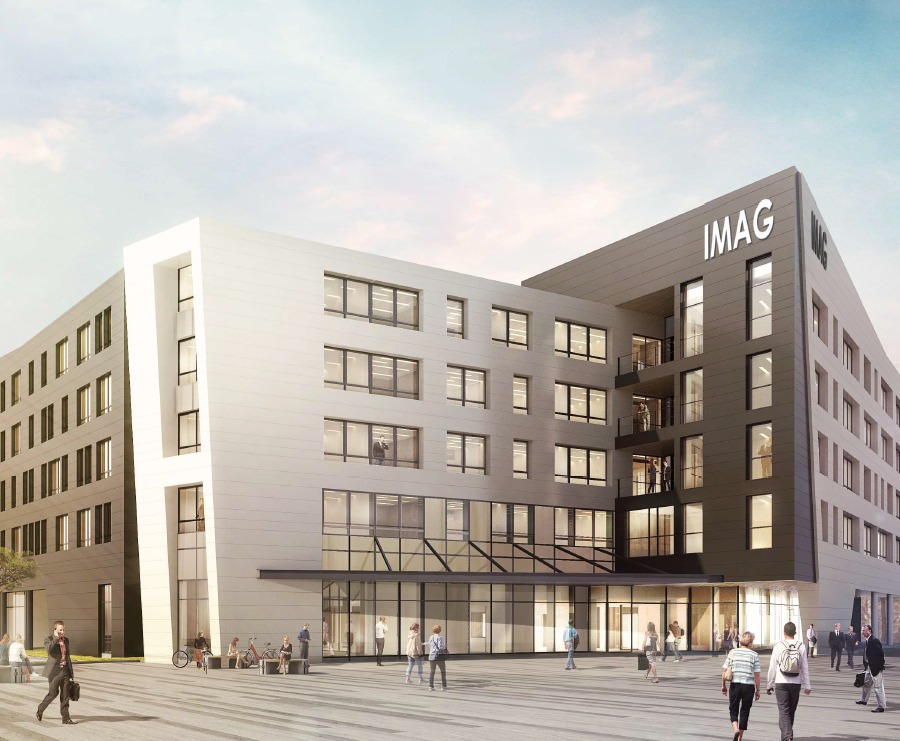
\includegraphics[width=0.8\textwidth,height=0.8\textheight,keepaspectratio]{images/imag.png}
\caption{bâtiment IMAG}
\end{figure}

Mon stage s'est déroulé au LIG ou laboratoire informatique de Grenoble,
ce laboratoire ainsi que certains autres sont situés dans le bâtiment
IMAG, situé au centre de Saint-martin-d'Heres. Il est le réceptacle de
nombreux projets de recherches et de recherche. Durant mon temps au LIG,
j'ai eu la possibilité de rencontrer de nombreux professionnels,
représentant des différents laboratoires présent dans le
bâtiment.\newline

Le bâtiment est organisé de la sorte :

\begin{itemize}
\item
  1er étage : AMIES, LJK, MAIMOSINE : \textbf{Mathématique}
\item
  2ème étage : GRICAD, LIG, VERIMAG : \textbf{Informatique}
\item
  3ème et 4ème étages: LIG : \textbf{Informatiques}\newline
\end{itemize}

Durant mon stage j'ai eu l'occasion d'assister à de nombreuses
conférences réalisées par des professionnels du sujet, comme une
conférence sur les FPGA ou sur les stratégies de test dans le monde du
HPC. J'ai aussi eu la chance d'animer un cours d'informatique débranché
destiné à deux classes de seconde, afin de les faire réfléchir sur des
problématiques d'informatique sans l'interférence d'un
ordinateur.\newline

En outre, mon stage au laboratoire ma permis de faire de nombreuses
découvertes et expériences en plus de toutes les connaissances que j'ai
pu accumuler.

\hypertarget{luxe9quipe-datamove}{%
\subsection{L'équipe DATAMOVE}\label{luxe9quipe-datamove}}

L'équipe de recherche \href{https://www.inria.fr/fr/datamove}{DATAMOVE}
du Laboratoire d'Informatique de Grenoble (LIG) se consacre à l'étude et
au développement de techniques innovantes dans le domaine du traitement
et de la gestion des données. Leur objectif est de relever les défis
liés à la croissance exponentielle des données et de proposer des
solutions efficaces pour leur manipulation, leur analyse et leur
exploitation.\newline

L'équipe est spécialisée dans les piles logicielles distribuées et
l'ordonnancement, généralement dans un environnement de High Performance
Computing. Dans ce laboratoire, le sujet de la \gls{reproductibilité}
est majeur grâce à la complexité des piles logiciels créées.\newline

La reproductibilité est une notion essentielle en recherche
\cite{reproductibility2017}, en effet cela consiste à pouvoir réaliser
une expérience à l'identique de la version d'origine afin d'obtenir le
même résultat. Cette approche permet de garantir l'intégrité et la
crédibilité des résultats scientifique. Il n'est cependant pas aisé de
rendre une expérience reproductible en informatique à cause de
l'omniprésence d'états qui peuvent être changés d'une exécution à une
autre. De plus, il peut y avoir des problèmes de version de logiciel,
disparition de ressource, d'accès au ressources de calcul ou encore la
présence d'une variable aléatoire. Tous ces problèmes, engendre un
problème de reproductibilité des logiciels.\newline

Dans le domaine du \Gls{hpc}, la reproductibilité présente plusieurs
avantages. Tout d'abord, elle permet de valider les méthodes de
modélisation et de simulation, garantissant ainsi que les résultats
obtenus sont fiables et précis, même si il peux être incorrect. Cela
renforce la confiance dans les résultats de recherche et facilite la
collaboration et la comparaison des résultats entre différents
chercheurs et laboratoires. De plus, dans ce genre d'environnement ou
les chercheurs déploie des simulations complexes avec des quantités
massives de données à analyser, il est essentiel que ces résultats
puissent être déterministes, ne serait-ce que pour pouvoir assurer de la
rigueur de la recherche.\newline

C'est dans cette optique que des outils de mise en place de pile
logicielle comme \Gls{nixos-compose} ont été mis en place dans
l'équipe.\newline

\textbf{L'équipe}\newline

En ce jour l'équipe DATAMOVE est composé de 34 personnes :

\begin{itemize}
\item
  10 chercheur.e.s
\item
  16 étudiant.e.s en thèse
\item
  5 ingénieurs
\item
  3 assistant.e.s\newline
\end{itemize}

Cette équipe est dirigée par Bruno RAFFIN. Olivier RICHARD, Quentin
QUILLOTEAU et Adrien FAURE sont tous membres de cette équipe.
Respectivement en tant que chercheur, étudiant en thèse et
ingénieur.\newline

\textbf{Quelques projets phares de l'équipe}\newline

\Gls{oar} est un gestionnaire de ressources distribuées conçu pour les
environnements de calcul intensif. Il permet aux chercheurs de
planifier, de contrôler, répondre et alloué des ressources demandé par
un utilisateur dans des environnements telles que les clusters de
calcul, les grilles de calcul et les infrastructures de cloud computing.
OAR offre une gestion fine des tâches, des files d'attente et des
politiques de priorité, permettant ainsi une utilisation efficace et
équitable des ressources. Cet outil facilite la planification des
travaux de recherche et optimise l'utilisation des infrastructures
informatiques. Cet outil est notamment utilisé dans Grid5000 pour la
réservation et l'allocation des ressources.\newline

Melissa, quant à lui, est un framework pour le développement
d'applications parallèles et distribuées. Il fournit une infrastructure
logicielle permettant aux chercheurs de concevoir et d'exécuter des
applications haute performance sur des environnements hétérogènes et
distribués. Melissa simplifie le processus de développement en
fournissant des abstractions de haut niveau pour la programmation
parallèle, l'orchestration des tâches et la gestion des données
distribuées. Cet outil permet aux chercheurs de tirer pleinement parti
des ressources informatiques disponibles et de développer des
applications performantes et évolutives.\newline

NixOS-Compose est un outil conçu pour les expériences dans les systèmes
distribués. Il permet de générer des environnements distribués
reproductibles afin d'être déployés sur une plateforme physique ou
virtualisé. C'est le logiciel auquel j'ai le principalement contribué et
utilisé lors de ce stage.

\newpage

\hypertarget{missions-au-sein-de-luxe9quipe-datamove}{%
\section{Missions au sein de l'équipe
DATAMOVE}\label{missions-au-sein-de-luxe9quipe-datamove}}

\hypertarget{lenvironnement-nix-et-nixos}{%
\subsection{L'environnement Nix et
NixOS}\label{lenvironnement-nix-et-nixos}}

\hypertarget{nix}{%
\subsubsection{Nix}\label{nix}}

\begin{figure}[h]
\centering

\includegraphics[width=0.2\textwidth,height=0.2\textheight,keepaspectratio]{logos/nixlogo.png}
\caption{Logo Nix}
\end{figure}

Nix a été la technologie clé de mon stage. C'est la technologie phare
que j'ai été amené à étudier et à comprendre tout au long de mon stage
au Laboratoire Informatique de Grenoble.\newline

Nix est un gestionnaire de paquet fonctionnel et un outil de déploiement
d'environnement reproductible. Il permet la gestion des dépendances
logicielles de manière déclarative et garantit la reproductibilité des
environnements de développement, et ce, en utilisant son propre langage,
le \emph{Nix Expression Language}, communément appelé Nix. Le langage
Nix est fonctionnel, pure à évaluation paresseuse. Comme dit
précédemment, le mot clé de Nix est reproductibilité. Son langage, sa
gestion des paquets et son architecture fonctionnelle lui permettent
d'obtenir un résultat toujours identique pour des conditions
identiques.\newline

\begin{figure}[h]
\centering
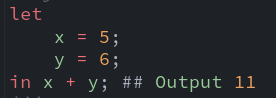
\includegraphics[width=0.8\textwidth,height=0.8\textheight,keepaspectratio]{images/codebasenixdark.png}
\caption{Code nix basique}
\end{figure}

La particularité de Nix réside dans son approche fonctionnelle. En
effet, Nix ne dépend pas de l'installation globale des paquets dans le
système d'exploitation. À la place, chaque paquet est traité comme une
fonction pure qui prend en entrée une version spécifique du paquet et de
ses dépendances et retourne en sortie une version spécifique du paquet.
Grâce à ce système, on met de côté le problème de \Gls{depedency-hell}
si commun dans la plupart des gestionnaires de paquet et l'on s'assure
que chaque paquet ait la version requise et demandée.\newline

Enfin, Nix est aussi capable de générer des environnements isolés
configurables. Il est possible de créer des environnements shell
possédant des dépendances spécifiques. Cela évite les conflits entre les
différentes versions d'un paquet utilisé par des applications, mais
aussi, permet de faciliter la portabilité, car une dépendance peut être
utilisée sans avoir été installé par l'utilisateur (c'est ce que j'ai
fait pour compiler ce rapport par exemple !).\newline

\textbf{Le Nix-Store}\newline

Le store Nix est un composant essentiel pour assurer le bon
fonctionnement et la reproductibilité du système de gestion de paquet
Nix. Il fonctionne sous forme de système de fichier hiérarchique qui
stocke tous les paquets présents dans la machine dans un dossier
spécifique nommé \texttt{store}. La gestion diffère donc des
gestionnaires de paquets classiques comme apt ou pacman qui stocke tout
en utilisant un système de fichier standard
(\texttt{usr/bin},\texttt{usr/lib}).\newline

Le store Nix repose sur 5 principes clés :

\begin{itemize}
\item
  \textbf{Hashing des paquets} : Chaque paquet ou dépendances dans le
  store est identifié par un hachage spécifique parfait basé sur ses
  entrées. Grâce à ce système, deux paquets identiques ne seront stockés
  qu'une seule fois. De plus, il est donc possible de stocker plusieurs
  versions d'un même paquet.
\item
  \textbf{Immutabilité des fichiers} : Les paquets présents dans le
  store sont immuables. Il est impossible d'en effectuer une
  modification après leur création. C'est un avantage considérable, car
  cela assure l'intégrité des paquets et limite les effets de bord
  néfaste.
\item
  \textbf{Liens symboliques} : Les fichiers, dossier et dérivations
  présent dans le store sont référencés par des liens symboliques,
  permettant au utilisateur de pouvoir utiliser les paquets présent dans
  le store sans avoir besoin de mettre à jour le PATH ou de connaitre le
  chemin exact (et donc le hash) du paquet.
\item
  \textbf{Gestion des dépendances} : Les paquets présents dans le store
  utilisent des liens symboliques référençant chaque dépendance qu'il
  possède. Cela permet de nous assurer que chaque paquet utilise la
  bonne version de chaque dépendance.
\item
  \textbf{Garbage Collection} : Enfin, le store possède un système de
  \gls{garbage-collection} basé sur des \emph{Garbage root}.
  C'est-à-dire que les paquets installés et donc devant être gardé sont
  stockées en tant que garbage root. À la garbage collection
  (\texttt{nix-collect-garbage}) les garbage root et leurs dépendances
  sont gardés et le reste est élagué par le système. Ce système est
  important, car chaque dépendance est téléchargée et stockée dans le
  store. Ce qui peut rendre le store très lourd.\newline
\end{itemize}

Tous ces principes permettent la reproductibilité des environnements de
développement ainsi que des paquets et application du système. On
s'assure donc une cohérence générale et une prédictibilité du
système.\newline

\begin{figure}[h]
\centering
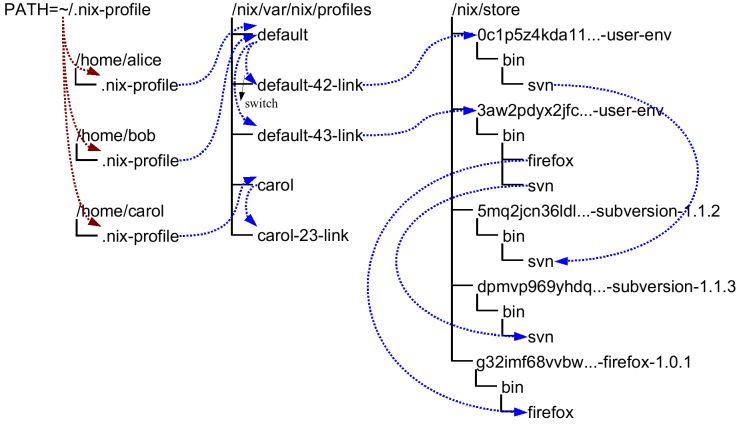
\includegraphics[width=0.8\textwidth,height=0.8\textheight,keepaspectratio]{images/store.png}
\caption{Exemple d'architecture de store multi utilisateur}
\end{figure}

Comme on peut le voir dans la figure 4, il est donc possible avec ce
système de posséder plusieurs subversion d'un même paquet. De plus, avec
le système de profil Nix, il est possible de définir quel utilisateur
utilisent quel paquet et donc séparer les utilisateurs. Cependant, peu
importe le nombre d'usagés de la machine, il n'y aura toujours qu'un
seul store global.\newline

\textbf{Les Nix Flakes}\newline

Les flakes sont une fonctionnalité encore expérimentale de Nix qui vise
à d'autant plus améliorer la reproductibilité, la modularité et la
gestion des dépendances dans Nix. Il permet de définir une interface
commune pour importation de ressource extérieure. Bien que toujours en
phase expérimentale, les flakes sont massivement utilisés par la
communauté grâce aux ajouts importants qu'il permet. Ils sont
régulièrement considérés par la communauté des utilisateurs de nix comme
un ajout essentiel au bon fonctionnement actuel de nix et à sa
prospérité.\newline

Afin de réaliser un flake, il suffit de créer un fichier
\texttt{flake.nix}. Un flake ne prend pas de paramètre d'entrée comme
pourrait le faire un script nix classique. À la place, il récupère des
ressources sous forme d'input et les utilisent pour y créer une sortie.
Ces paramètres d'entrées peuvent être un dépôt distant Git ou un autre
flake par exemple.\newline

Comme il ne prend pas de paramètre d'entrée, il ne dépend aucunement de
la configuration de la machine actuelle. À la compilation, un flake crée
un fichier \texttt{flake.lock} qui définie les versions, le type du
dépôt, la dernière date de modification, etc. Ce fichier permet donc
d'avoir une trace des versions utilisées et de pouvoir les réutiliser de
la même manière. Ce système est appelé \gls{pinning}.\newline

En outre, les nix flakes est un élément essentiel à Nix et est une
technologie que j'ai massivement utilisée lors de mon stage et qui est
utilisée dans de nombreux systèmes tels que NixOS-Compose par
exemple.\newline

\textbf{Exemple d'environnement nix}\newline

\begin{figure}[h]
\centering
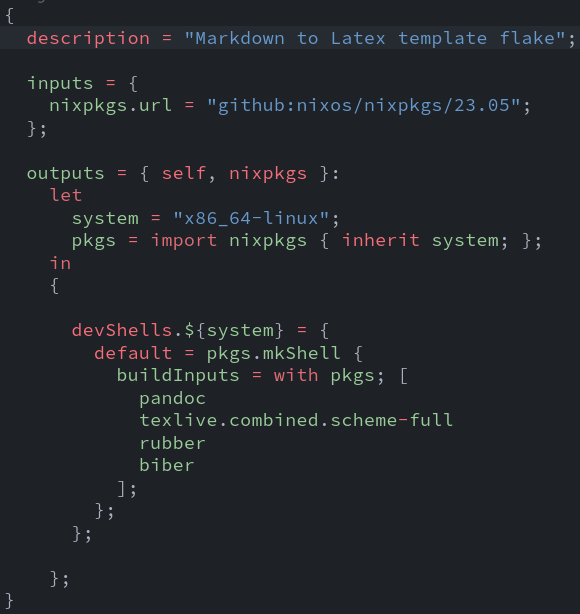
\includegraphics[width=0.8\textwidth,height=0.8\textheight,keepaspectratio]{images/flakebasenix.png}
\caption{Script nix de creation d'environnement latex}
\end{figure}

Voici un exemple de création d'environnement isolé Nix en utilisant les
flakes Nix. Ce script ne marche que sur les architectures
\texttt{x86\_64-linux}, car il ne récupère les dépendances que de cet
ordinateur. Ce script rajoute dans la PATH du terminal en cours les
applications mise dans les \texttt{buildInputs}, c'est-à-dire dans ce
cas \texttt{pandoc}, \texttt{rubber} et \texttt{biber}. À la fin de
cette session, le PATH sera remis à défaut. Pour l'exécuter, il faut
effectuer la commande \texttt{nix\ develop\ .} ou ``.'' est le chemin
vers le flake. C'est ce genre de configuration que j'ai été amené à
utiliser et à créer afin d'avoir un environnement et un résultat
reproductible.\newline

\hypertarget{nixos}{%
\subsubsection{NixOS}\label{nixos}}

NixOS est une distribution Linux entièrement basé sur Nix. Il utilise
une approche déclarative pour effectuer la configuration système.
L'intégralité de la configuration est définie par le biais du fichier
\texttt{configuration.nix}. C'est un principe très agréable, car cela
permet de très simplement stocker et versionner la configuration du
système afin de pouvoir par exemple la réutiliser dans une architecture
similaire.\newline

NixOS utilise Nix pour s'occuper de la gestion des paquets. Donc, chaque
paquet est traité manière fonctionnelle. NixOS suit un modèle de mise à
jour sous le nom de \emph{Rolling Release}. Cela consiste à fournir des
mises à jour de manière incrémentale et régulière. Dans le cas de NixOS,
tous les 6 mois. Enfin, le système d'exploitation stocke la
configuration système après chaque changement, permettant de retourner à
tout moment à une configuration précédente en cas de problème.\newline

Pour résumer, NixOS est un Système d'Exploitation innovant et sûr, je
suis ravie d'avoir réalisé l'intégralité de mon stage dans cet
environnement, sur une machine dédié. Cette utilisation intensive de cet
OS m'a permis de développer des compétences système importantes. Le
Système d'Exploitation NixOS a été pour moi une très belle
surprise.\newline

Cependant, il n'est évidemment pas parfait. NixOs utilisant un système
de \emph{Rolling Release} semestriel, il faut souvent réparer la
configuration du système qui s'est vu être modifié par la mise à jour.
De plus, le store Nix propose beaucoup d'atout, mais n'est pas très
efficace quand il faut mettre à jour des paquets régulièrement, comme
Visual Studio Code par exemple. Le store étant immuable, il faut donc
forcer la configuration à utiliser une source plus récente si l'on veut
une version stable de l'application utilisée.\newline

\hypertarget{nixpkgs-et-nur-kapack}{%
\subsubsection{Nixpkgs et Nur-Kapack}\label{nixpkgs-et-nur-kapack}}

Nixpkgs et NUR (Nix User Repository) sont des dépôts de paquets Nix. Ils
sont utilisés massivement le gestionnaire de paquet, en tant que
collection de paquet et logiciel installable par les utilisateurs
possédant Nix. Durant mon stage, j'ai eu la possibilité de rajouter des
paquets dans certain de ces dépôts, afin qu'il soit utilisable par la
communauté Nix.\newline

\textbf{Nixpkgs}\newline

\href{https://github.com/NixOS/nixpkgs}{Nixpkgs} est le dépôt principal
de paquet Nix, il est automatiquement référencé en tant que tel dans une
machine NixOS. Il contient l'un des plus grands nombres de paquets pour
un package manager. plus de 80 000. Ces paquets peuvent être des outils
de développement, des bibliothèques, des applications, etc. Les paquets
disponibles sont ajoutés et maintenus par la communauté et sont
constamment mis à jour afin d'assurer que les logiciels soient toujours
dans une version correcte. Ce qui permet à Nix d'être la distribution la
plus à jour.\newline

\textbf{NUR}\newline

Nur est un dépôt de paquet supplémentaire à Nix, il est maintenu par des
utilisateurs ou des membres de la communauté. Contrairement à Nixpkgs,
tout le monde peut déposer des paquets dans Nur. Grâce à ce dépôt, il
est donc possible de partager des paquets spécifiques et de les rendre
disponible à la communauté. Nur, est donc une alternative qui permet de
compléter Nixpkgs.\newline

Le fonctionnement de ces outils dépend de la collaboration de la
communauté. Cette collaboration permet à Nix de posséder le plus grand
nombre de paquets disponible dans un gestionnaire de paquet. Et ce de
manière fonctionnel. C'est un élément essentiel de la réussite de Nix et
NixOS.\newline

Durant ce stage, j'ai rajouté des paquets dans des dépôts, afin de les
rendre utilisable par la communauté. Notamment sur le dépôt
\href{https://github.com/oar-team/nur-kapack}{Nur-kapack} un sous dépôt
de NUR, créé par l'équipe DATAMOVE pour y stocké les paquets important
pour la recherche au laboratoire. J'ai eu l'occasion de comprendre son
fonctionnement, tester certain des paquets et donc y rajouter des
fonctionnalités et des paquets.

\newpage

\hypertarget{les-outils-uxe0-disposition-pour-la-recherche}{%
\subsection{Les outils à disposition pour la
recherche}\label{les-outils-uxe0-disposition-pour-la-recherche}}

La communication est un élément essentiel au bon fonctionnement d'une
équipe de recherche. Il est donc nécessaire dans ce type d'encadrement
d'utiliser des outils adapté et efficace afin de pouvoir communiquer
avec les autres membres du laboratoire et potentiellement pour pouvoir
poser des questions à propos de certaines technologies.\newline

\textbf{Mail}\newline

Le système de mail était important pour le bon fonctionnement du LIG. Il
était vecteur de message et d'information essentiel pour tous les
membres du laboratoire. J'avais à ma disposition une adresse mail INRIA.
Les mails sont particulièrement importants afin de recevoir des
informations pour les prochaines conférence et séminaire présent dans le
bâtiment IMAG. Ces conférences ont été importantes, car elles étaient
vectrices de nombreuses connaissances et permettait d'exacerber ma
curiosité sur le domaine de l'informatique en général.\newline

\textbf{Telegram}\newline

Le réseaux de communication Telegram était utilisé par l'équipe de
recherche afin de pouvoir créer des salons de discussion sur des
domaines précis. Ce moyen de communication est bien plus rapide et moins
formel que l'utilisation de mail. Ce qui permet de facilité la
discussion entre les membres de l'équipe.\newline

\textbf{Gitlab et Github}\newline

L'utilisation d'un gestionnaire de version git est une évidence et
parfaitement essentiel dans n'importe quel type de projet informatique.
Il permet de s'assurer de la pérennisation du code. Lors de mon stage,
j'ai utilisé massivement le Gitlab de l'Inria afin d'y entreposé les
dépôts que j'ai créés pour chacune de mes compositions. J'ai également
fait partie du groupe de développeur oar sur GitHub. Ce système ma
permis de centraliser la documentation que j'ai écrite. Enfin, git
permet de communiquer et de discuter de certain problème par le biais
des issues git. Les issues sont une partie essentielle du bon
fonctionnement d'un projet, surtout dans un domaine si précis que celui
de la recherche.

Voici les projet que j'ai plus particulièrement contribué :

\begin{itemize}
\item
  \href{https://github.com/oar-team/nur-kapack}{Nur-Kapack}
\item
  Rajout de composition de Files System distribué dans le
  \href{https://gitlab.inria.fr/nixos-compose/hpc-io}{groupe HPC-IO}
\item
  \href{https://gricad-gitlab.univ-grenoble-alpes.fr/regale/tools/regale-nixos-compose}{Regale}
\item
  \href{https://gitlab.inria.fr/nixos-compose/nixos-compose}{NixOS-Compose}
\item
  Le \href{https://gitlab.inria.fr/nixos-compose/stages/alithaud}{dépot
  de stockage des ressources du stage}
\end{itemize}

\newpage

\hypertarget{loutil-nixos-compose}{%
\subsection{L'outil NixOS-Compose}\label{loutil-nixos-compose}}

\Gls{nixos-compose} (ou NXC) est l'outil principal que j'ai utilisé
durant mon stage. C'est un outil de déploiement d'environnement
distribué, reproductible et éphémère.\newline

\begin{figure}[h]
\centering
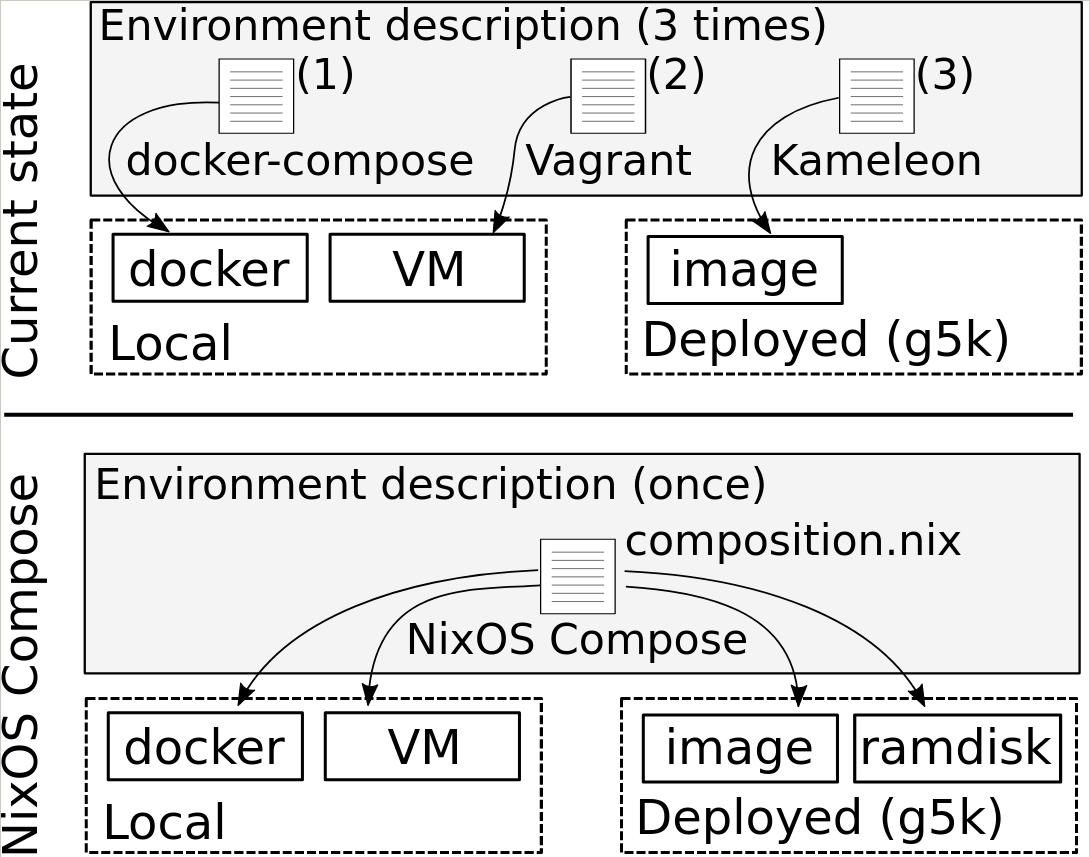
\includegraphics[width=0.8\textwidth,height=0.8\textheight,keepaspectratio]{images/shema-nxc.png}
\caption{Schéma de fonctionnement de NXC}
\end{figure}

NixOS-Compose permet de créer de déployer des compositions, c'est-à-dire
une description fonctionnelle d'un environnement distribué. Une
composition est une description d'une architecture distribuée, et ce, de
manière fonctionnel. En effet, chaque composition est écrite en
utilisant le langage de programmation Nix. Une composition permet de
décrire plusieurs \textbf{rôles}. Ces rôles correspondent à une
configuration d'une machine NixOS. Il est donc possible grâce à cet
outil de déployer directement un environnement de machines distribuées
configuré en utilisant NixOS d'une façon spécifique et
déclarative.\newline

\begin{figure}[h]
\centering
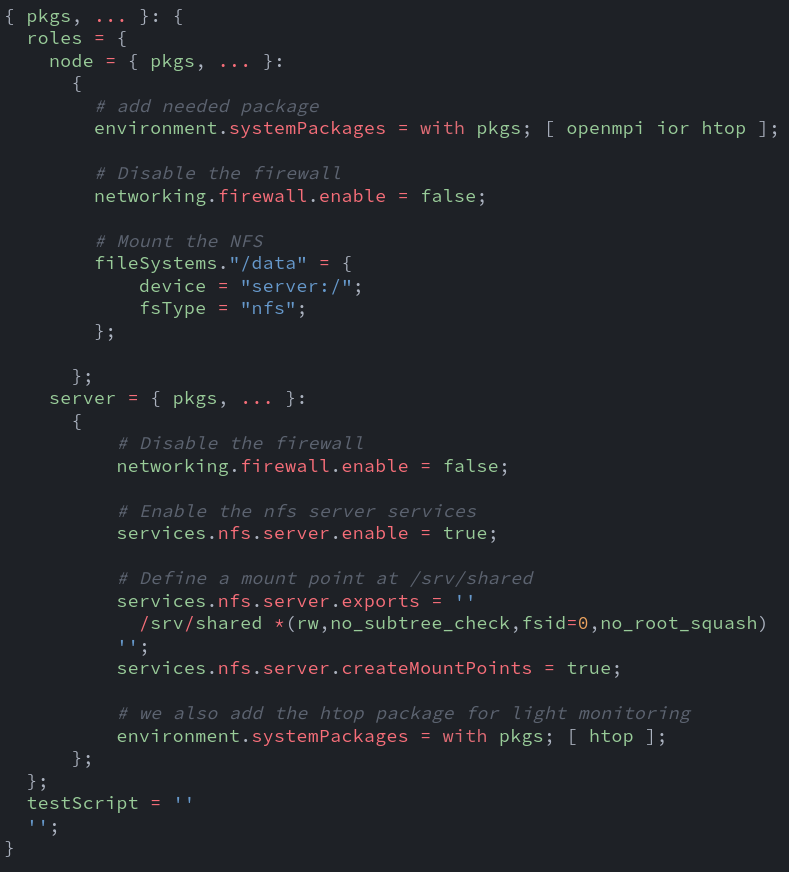
\includegraphics[width=0.8\textwidth,height=0.8\textheight,keepaspectratio]{images/coposition-nfs.png}
\caption{Exemple de composition}
\end{figure}

La figure 7 correspond à un exemple simple de composition Nix dans
lequel nous créons 2 rôles différents : \texttt{node}, \texttt{serveur}.
Le node possède des outils de calcul de performances, ior et htop. Le
server quant à lui initialise le service \texttt{nfs}, de partage de
fichier, qui est présent dans le langage Nix car créé par la communauté
dans le dépôt nixpkgs.\newline

Chacun de ces rôles sont configurés en utilisant le Nix et permettent en
quelques lignes de créer deux noeuds, directement en communication, et
ce, de manière éphémère et reproductible. Il semble donc évidement de
comprendre l'intérêt d'un tel outil dans le monde la recherche. La
création simple de noeud reproductible et éphémère permet de créer des
conditions de recherche optimal, et ce, dans de nombreuses
conditions.\newline

\textbf{Le déploiement}\newline

À la fin de la compilation de la composition (commande
\texttt{nxc\ build}), NXC créer un fichier json stockant en son sein les
informations importantes pour chaque rôle. L'utilisateur est libre du
nombre de noeud ou machines qui vont utiliser la configuration d'un
rôle. Ainsi, dans l'exemple de la figure 7 il est possible à
l'utilisateur de choisir lu nombre de machines utilisant le rôle
\texttt{node} ou \texttt{serveur}, et ce sans avoir besoin de recompiler
les rôles.\newline

À la base, il faillait directement définir le nombre de noeud voulu dans
la composition. Cette solution, bien que très fonctionnel, force
l'utilisateur de recompiler à chaque changement de cette valeur, ce qui
est une perte sèche de performance.\newline

Maintenant, il est possible de déployer (commande \texttt{nxc\ start})
directement le nombre de machines voulu à la phase de déploiement par le
biais d'un fichier YAML (\emph{YAML Ain't Markup Language}). Cette
amélioration permet d'augmenter massivement les performances de NXC lors
de calcul de performance par exemple, car le test ne va devoir compiler
que les rôles NXC de base et déployer les noeuds.\newline

\textbf{Les flavours}\newline

Comme vu dans la figure 6, NixOS-Compose permet en plus de déployer les
compositions écrites dans plusieurs environnements différent, choisi
lors du build de la composition. Ces différents choient d'environnement
de déploiement sont appelés des flavours.\newline

Il existe un certain nombre de flavours disponible avec NixOS-Compose
:\newline

\begin{itemize}
\item
  \textbf{VM}, qui créer une image locale utilisable dans un système de
  machine virtuelle QEMU.
\item
  \textbf{Docker}, qui créer un système de conteneurisation en utilisant
  Docker et Docker-Compose.
\item
  \textbf{G5K-ramdisk}, qui va créer une image ramdisk, et donc va
  stocker en sen sein l'intégralité du store, ce qui rend cette
  technique très lourde.
\item
  \textbf{G5K-nfs-store}, qui va utiliser nfs pour faire du partage de
  paquet dans le store nix et donc limiter la taille globale de l'image.
\item
  \textbf{G5K-image}, qui va créer une image déployable selon des
  configurations différentes.\newline
\end{itemize}

Les flavours G5K sont celle qui est utilisables dans l'environnement
Grid5000 qui utilise Kameleon pour pouvoir créer et déployer de cette
architecture.\newline

Il est donc possible de tester des compositions sur plusieurs
environnement afin de pouvoir s'assurer du bon fonctionnement du système
et de calculer les performances dans des conditions différentes. Les
flavours sont un point essentiel de l'importance de l'outil
NixOS-Compose.\newline

\textbf{Les test NixOS}\newline

NixOS possède un système de test unitaire capable de définir un
environnement dans un fichier de configuration et d'utiliser des scripts
python afin de pouvoir tester le fonctionnement de ce système. Ce type
de fichier est commun et couramment utilisé dans la communauté Nix. De
nombreux fichiers de tests unitaires sont disponibles dans le dépôt de
paquet
\href{https://github.com/NixOS/nixpkgs/tree/master/nixos/tests}{Nixpkgs}.\newline

Les compositions NixOS-Compose réutilisent la structure pré-établie par
les tests NixOS. Cela permet de facilement passé de Test NixOS à
composition NXC afin de pouvoir rapidement tester une technologie dans
un environnement distribué. En effet, la syntaxe des tests sont
similaires et servent généralement de base à la composition s'ils sont
présents dans nixpkgs. NixOS-Compose reprend donc pour ces compositions
la syntaxe des tests, mais NXC permet de répondre à des problèmes que
les tests NixOS seraient incapables de réaliser.\newline

Le lien avec ces tests permet à NixOS-Compose d'être plus accessible
pour la communauté des utilisateurs de Nix en plus de facilité la
transition entre test simple et composition avancé.\newline

J'ai été amené à utiliser et à comprendre le fonctionnement de chacune
des particularités de cet outil tout au long de ce stage.\newline

\newpage

\hypertarget{duxe9veloppement-de-composition-nixos-compose}{%
\subsection{Développement de Composition
NixOS-Compose}\label{duxe9veloppement-de-composition-nixos-compose}}

\hypertarget{fonctionnement-et-composition-simple}{%
\subsubsection{Fonctionnement et Composition
Simple}\label{fonctionnement-et-composition-simple}}

\hypertarget{workflow}{%
\subsubsection{Workflow}\label{workflow}}

\hypertarget{grid5000}{%
\subsubsection{Grid5000}\label{grid5000}}

Grid5000 (ou G5K) est une infrastructure de recherche expérimentale
dédiée aux systèmes distribués. Il a joué un rôle crucial pour moi tout
au long du stage. Plus précisément, il s'agit d'un réseau de machines ou
clusters hébergés un peu partout en France. Permettant de réserver et
d'utiliser des machines hautes performances rapidement en utilisant une
connexion ssh.

Grid5000 est ce qu'on peut appeler un \emph{testbed}, ou banc de test
pour la recherche française et internationale.\newline

\begin{figure}[h]
\centering
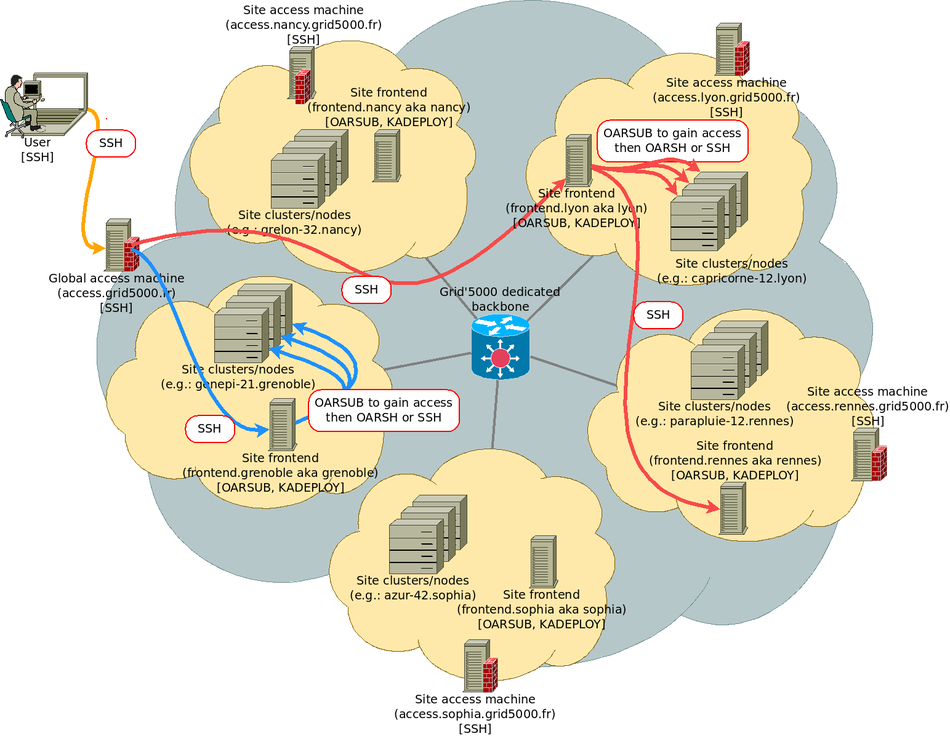
\includegraphics[width=0.8\textwidth,height=0.8\textheight,keepaspectratio]{images/shemag5k.png}
\caption{Schema de Grid5000}
\end{figure}

Comme visible dans la figure ci-dessus, la connexion ssh de Grid5000
donne l'accès à la machine centrale à tous les utilisateurs du site
choisi, cette machine est appelée la frontale. Elle contient en son sein
l'intégralité des espaces de stockage de chaque utilisateur. Il est
important pour le bon fonctionnement de ne pas demander à la frontale de
faire des calculs intensifs, car cela causerait des ralentissements pour
tous les utilisateurs. \newline

Comme Grid5000 utilise ssh, j'ai été amenée à utiliser et à comprendre
l'outil tmux. Tmux est un multiplexeur de terminal qui permet par son
implémentation de sauvegarder des sessions de terminal. C'est un outil
très intéressant que j'utilise toujours aujourd'hui sur mon ordinateur
personnel. Ce multiplexeur de terminal était particulièrement important
avec grid5000, car son système de session permet de récupérer une
connexion ssh en utilisant la commande \texttt{tmux\ attach} ou
\texttt{tmux\ a} afin de récupérer la session perdue. Cela m'a permis
d'éviter de perdre beaucoup de temps lors de l'utilisation de
G5K.\newline

Afin d'utiliser Grid5000, il faut utiliser les commande OAR dans le but
de demander des noeud au système, le scheduler OAR donnera accès au
nombre de machines voulu selon la place restante dans le cluster. Pour
réserver des noeuds les utilisateurs utilisent la commande
\texttt{oarsub}.

Voici un exemple de commande oar qui va réserver 42 noeuds pendant 3h20
:

\begin{verbatim}
oarsub -l nodes=42,walltime=3:20:0
\end{verbatim}

\begin{figure}[h]
\centering
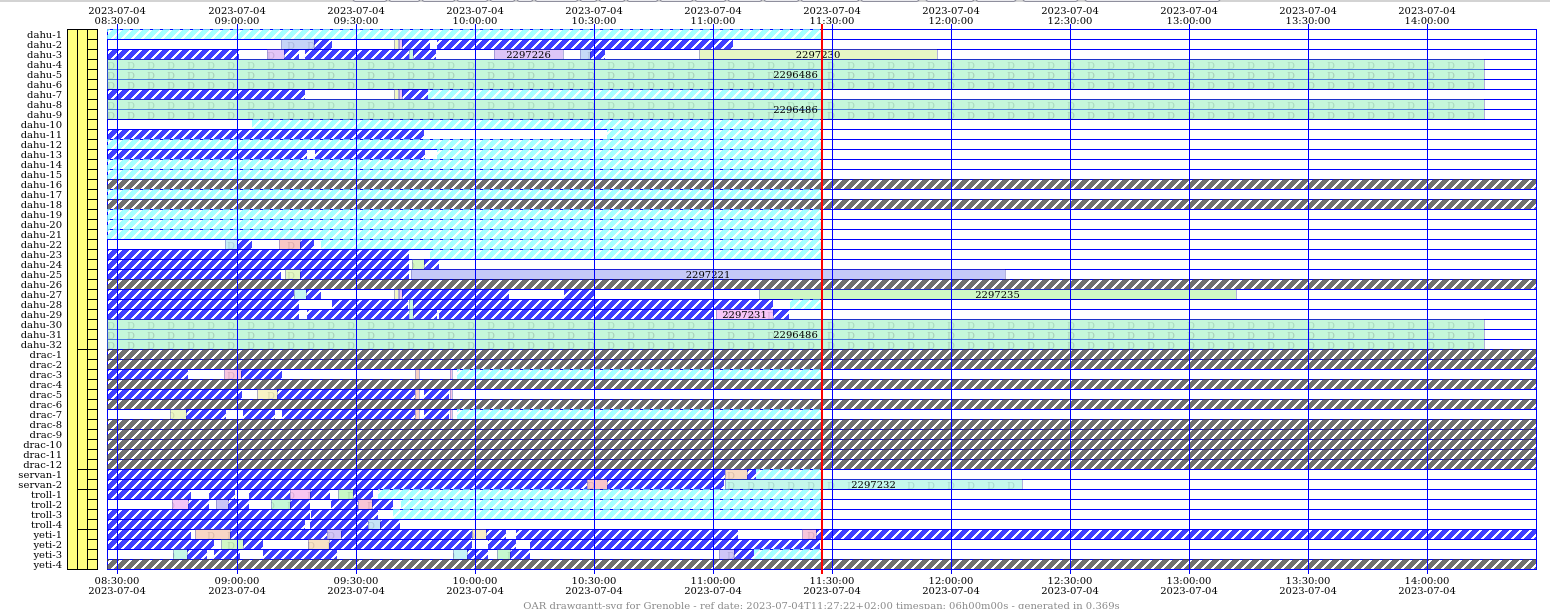
\includegraphics[width=0.8\textwidth,height=0.8\textheight,keepaspectratio]{images/ganttg5k.png}
\caption{Diagramme de Gantt d'utilisation des noeuds de Grid5000 en temps réel}
\end{figure}

Durant mon stage, j'ai massivement utilisé le système Grid5000 afin de
pouvoir build et surtout déployer mes compositions NixOS-Compose. En
effet, certaines compositions que j'ai créées étaient massives et
nécessitaient énormément de temps de calcul au build pouvais nécessiter
une dizaine de machines. Il était inconcevable de simuler cette
architecture sur mon ordinateur possédant uniquement 8 Go de RAM. Mon
ordinateur était simplement incapable de simuler de grandes expériences
distribuées. J'ai donc utilisé des flavours locale afin de faire des
tests simples et j'ai grandement utilisé Grid5000 pour simuler des
expériences beaucoup plus poussées sur les technologies que j'ai
implémenter sur NXC.\newline

\begin{figure}[h]
\centering
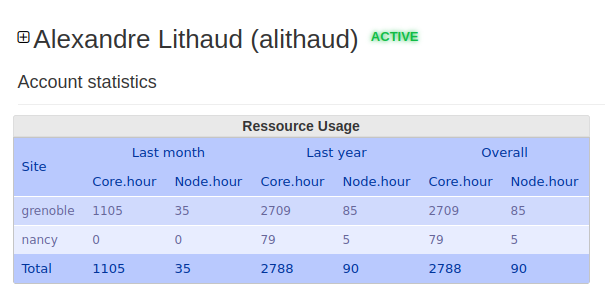
\includegraphics[width=0.8\textwidth,height=0.8\textheight,keepaspectratio]{images/statg5k.png}
\caption{Mes Statistiques d'utilisaion de Grid5000}
\end{figure}

Enfin, certaines des compositions que j'ai créées nécessitait la
modification ou l'ajout de système de fichier dans certain des noeuds or
cette action n'était possible que dans le système grid5000. En effet,
les flavours ``locale'', comme VM ou Docker n'utilise pas de disque, à
la place tout est stocké dans un file system temporaire qui
correspondait à la RAM attribuée. C'était un problème, car il était
impossible de modifier ou de rajouter de files system.

Cependant, chaque noeuds sur Grid5000 possède plusieurs disques.
Certains sont immuables et ne doivent pas être modifié sous risque de
voir le noeud s'arrêter. Mais il existe un disque nommé TMP qui était
utilisable et modifiable à souhait, car réinitialisé à chaque nouvelle
utilisation. C'est justement pour ce cas d'utilisation que ce disque est
présent dans chaque machine Grid5000. Il m'a donc suffi de chercher dans
les \texttt{partlabel} des disques de la machine et de regarder le label
du disque TMP.\newline

\begin{figure}[h]
\centering
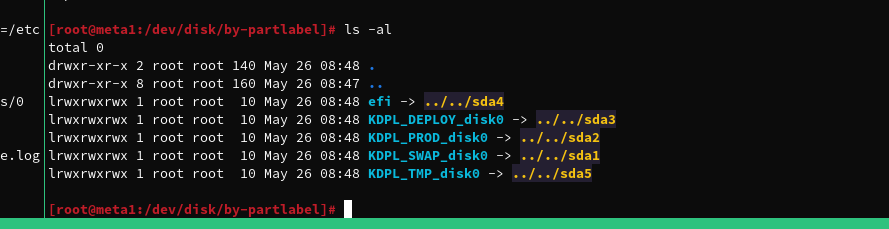
\includegraphics[width=0.8\textwidth,height=0.8\textheight,keepaspectratio]{annexe/disk_g5k.png}
\caption{disk-bypartlabel dans un noeud Grid5000}
\end{figure}

J'ai donc pu savoir quelle partition j'avais le droit de modifier et ai
pu finir le test de mes compositions sans problème.\newline

Grid5000 a donc été une partie essentielle de mon stage, car cela m'a
permis de pouvoir faire des expériences à grande échelle et de pouvoir
assurer le bon fonctionnement de mes compositions tout en permettant
d'échapper à quelques contraintes de fonctionnement des flavours
``locale'' NixOS-Compose.\newline

\hypertarget{file-systems}{%
\subsubsection{File Systems}\label{file-systems}}

\hypertarget{mes-contributions-au-projet}{%
\subsubsection{Mes contributions au
projet}\label{mes-contributions-au-projet}}

\newpage

\hypertarget{perspective-du-projet-nixos-compose}{%
\subsection{Perspective du projet
NixOS-Compose}\label{perspective-du-projet-nixos-compose}}

NixOS-Compose est un outil très puissant dans l'optique de créer et de
simuler des environnements reproductibles. La reproductibilité étant un
aspect omniprésent et essentiel de la recherche informatique, et ce,
dans tous les domaines, il semble raisonnable de penser que NXC aura un
avenir certain dans le monde de la recherche. Cependant, l'outil est
encore en développement et de nouvelles fonctionnalités seront à coup
sûr ajouté dans le futur.

Après ces quelques mois d'utilisation de l'application et de
développement de composition, voici les perspectives que j'envisagerai
pour NixOS-Compose.\newline

\textbf{Amélioration de certaines fonctionnalités}\newline

NixOS-Compose peut encore voir certaines de ces fonctionnalités
améliorer, par exemple, il peut être intéressant de pousser encore plus
les fonctionnalités du CLI NXC. Le CLI correspond à toutes les commandes
utilisables par l'outil NixOS-Compose, comme \texttt{nxc\ build},
\texttt{nxc\ init}, \texttt{nxc\ connect}, \texttt{nxc\ start},
\texttt{nxc\ driver}. Il serait intéressant de rajouter des
fonctionnalités comme la présence d'un \texttt{nxc\ check} qui a été
proposé et qui permettrait d'évaluer une composition sans la build, ce
qui faciliterait les tests de fonctionnement d'une composition. Avec
NixOS-Compose on essai de ``cacher'' la présence du Nix pour les
personnes voulant déployer des environnements. Cependant, on pourrait
imaginer pouvoir utiliser les templates Nix directement dans NXC en
utilisant l'option \texttt{-t} de \texttt{nxc\ init}.\newline

La fonctionnalité principale de NixOS-Compose consiste au déploiement
d'architecture de machine distribué dans différent environnement. En ce
moment, NXC est capable de déployer en local en utilisant des conteneurs
et des vm ou sur Grid5000. Il est donc essentiel pour la pérennité de
l'outil de rajouter des flavours afin de pouvoir déployer des
environnements reproductible sur des plateformes différentes. On peut,
par exemple, imaginer une implémentation d'OpenStack dans le but de
pouvoir créer une flavour de déploiement dans Kubernetes. C'est à mon
sens l'élément essentiel de développement de NixOs-Compose.\newline

Il pourrait être censé d'imaginer ajouter des outils à NixOS-Compose.
Ces outils pourraient être aussi être créé par des équipes de recherche.
C'est ce qui est proposé en ce moment avec l'outil enosLib.\newline

Actuellement NixOS-Compose utilise un noeud pour chaque rôle à déployer,
une proposition d'amélioration pourrait consister de créer un système de
\emph{folding} dans l'outil, similaire à ce que OAR peut déjà faire
actuellement. Ce principe de folding consiste à déployer un certain
nombre de rôles dans des machines virtuelles situé dans un noeud spécial
de ``calcul'' unique. Cette amélioration pourrait sans doute augmenter
les performances et réduire les consommations énergétiques des outils de
recherches utilisant NXC.\newline

\textbf{Amélioration de la Documentation et des Tutoriaux}\newline

La documentation est une partie essentielle d'un projet informatique. Il
permet de solidifier des connaissances et des maîtrises ainsi que
facilité l'utilisation des outils par des membres extérieurs.
NixOS-Compose possède une
\href{https://nixos-compose.gitlabpages.inria.fr/nixos-compose/}{documentation}
expliquant le fonctionnement général de l'outil ainsi que le workflow
général de l'application. Il serait donc une bonne amélioration de
remettre au bout du jour la documentation qui commence peux à peu à être
déprécié.\newline

NixOS-Compose possède également des
\href{https://gitlab.inria.fr/nixos-compose/tuto-nxc}{tutoriaux}, qui
permet de facilement pouvoir tester le fonctionnement de l'outil. Ces
tutoriaux sont essentiels, il serait donc une bonne chose de les
améliorer afin de rentrer encore plus dans les détails et de les mettre
à jour. \newline

Enfin, il faudrait à mon sens, dans l'optique de rendre l'utilisation de
NixOS-Compose la plus facile possible pour les nouveaux utilisateurs,
continuer de faire une documentation complète sur comment réaliser des
compositions efficaces. J'ai eu le plaisir de pouvoir commencer ce
document. Cependant, je n'ai malheureusement pas pu être exhaustif sur
les cas d'utilisation de cet outil à cause de sa complexité.\newline

\textbf{Intégration dans l'écosystème Nix}\newline

Finalement, la dernière perspective que je peux imaginer serai de
rajouter le NixOS-Compose dans nixpkgs. Actuellement NXC est présent
dans NUR. Cependant, en rajoutant l'outil dans nixpkgs, on assurerait
une intégration de NixOS-Compose directement dans l'écosystème Nix et
donc dans le système d'exploitation NixOS par la même occasion. Cela
pourrait permettre de rendre l'utilisation de NXC plus commune et plus
simple pour toutes les personnes voulant utiliser cette
technologie.\newline

\newpage

\hypertarget{conclusion}{%
\section{Conclusion}\label{conclusion}}

\hypertarget{bilan-personnel}{%
\subsection{Bilan personnel}\label{bilan-personnel}}

Ce stage m'a permis de découvrir le monde de la recherche de manière
poussé. De plus, j'ai développé une méthode de travail efficace. J'ai
découvert les problématiques qu'une équipe de recherche telle que
DATAMOVE peuvent poser.

Ce stage m'a permis de rencontrer des experts dans le sujet. Ces
interactions ont été essentielles tout au long du stage. Ainsi, elle
était le vecteur de nouvelles connaissances et de la découverte de
nouveaux outils qui font maintenant partie de mon quotidien d'ingénieur
(zsh, obsidian, fzf, tmux, \ldots) en plus de découvrir des nouvelles
méthodes de travail adapté au travail et efficace.

J'ai eu le plaisir de contribué à l'évolution de NixOS-Compose et de
découvrir des technologies puissantes comme Nix et NixOS qui m'ont
permis de m'améliorer sur des concepts important dans l'informatique
actuel comme le calcul de performance, la reproductibilité et le
déploiement de système distribué.\newline

\hypertarget{bilan-professionnel}{%
\subsection{Bilan professionnel}\label{bilan-professionnel}}

Sur un plan professionnel, ce stage m'a permis de découvrir et
d'expérimenter le travail en laboratoire. Ainsi que les spécialités du
travail dans une équipe de recherche tel que DATAMOVE.

J'ai grandement apprécié le système de fonctionnement de l'équipe. En
effet, dans cet environnement de travail, l'entraide et la communication
était omniprésente. J'ai donc eu le plaisir de développer au sein de
l'équipe des compétences de travail d'équipe et de coordinations avec
les différents membres du laboratoire. De plus, les différents
séminaires assistés et tâche réalisés me permirent de développer ma
curiosité notamment dans le domaine système de l'informatique tout en
développement mon bagage de connaissance et mon expérience technique.

Toutes ces expériences me seront à coup sûr très utiles et valorisant
dans le projet professionnel de DevOps que je souhaite entreprendre.

Je suis reconnaissant d'avoir eu la possibilité de contribué à ce projet
en y rajoutant des compositions qui pourront servir de base recherche
sur le calcul de performance de File System Distribués dans une
plateforme expérimentale tel que Grid5000. Je suis heureux d'avoir aidé
à la maintenance et au bon fonctionnement général de l'outils
NixOs-Compose qui sera sans aucun doute d'un importance majeur dans la
cadre de la recherche.\newline

\newpage

\hypertarget{annexe}{%
\section{Annexe}\label{annexe}}

\printbibliography

\printglossaries

\begin{titlingpage}
\newpage
\makefooter
\end{titlingpage}

\end{document}
